
\section{Ablation Study}
\label{sec:ablation}

To validate the design decisions underlying the PoP consensus mechanism, we vary four key parameters that govern the consensus pipeline---peer discovery depth, broadcast size, signature threshold, and collection timeout---and measure their impact on both \emph{consensus reliability} and \emph{operational cost}. For each configuration, we report two complementary views: (i)~the consensus status distribution (\texttt{CONFIRMED}, \texttt{INSUFFICIENT\_CONSENSUS}, \texttt{SINGLE\_WITNESS}) as the reliability metric, and (ii)~P2P message count plus wall-clock time as cost metrics. All experiments use the 200-AS CAIDA topology (126 RPKI observers) with default parameters unless the ablated variable is specified.

% =======================
% Parameter Sensitivity Analysis
% =======================
\subsection{Parameter Sensitivity}
\label{subsec:parameter_sensitivity}

All system hyperparameters are externalized in a single configuration file (\texttt{.env}) and loaded at startup, allowing operators to tune behavior without modifying source code. Table~\ref{tab:hyperparameters} lists the key parameters, their default values, and their effect on system behavior. We highlight three parameters whose settings most significantly influence experimental outcomes.

\textbf{Route Flapping Threshold (\texttt{FLAP\_THRESHOLD}).} This parameter controls how many unique state changes within a 60-second window trigger a ROUTE\_FLAPPING classification. At the default value of~5, the detector achieves high recall (catches all true flapping) but generates substantial false positives on legitimate prefixes with frequent updates: across our six datasets, false positives were recorded for route flapping, compared to zero false positives for the other three attack types (Table~\ref{tab:system_performance}). Increasing the threshold reduces false positives at the cost of potentially missing subtle flapping attacks. This trade-off is inherent to heuristic-based flapping detection and is well-studied in the BGP operations literature~\cite{rfc2439}.

\textbf{Consensus Timeout (\texttt{P2P\_REGULAR\_TIMEOUT}).} The 15-second default timeout for signature collection bounds the time each transaction waits for peer endorsements. At smaller scales (50~ASes), a higher fraction of transactions achieve full consensus within this window. At larger scales, the commit rate drops because more validators compete for the limited signature slots within the timeout. Increasing the timeout would improve commit rates but add latency; decreasing it would improve throughput at the cost of more single-witness commits. Critically, \emph{no data is lost} regardless of timeout setting: timed-out transactions are committed with their actual consensus status (Section~\ref{sec:architecture}), preserving every observation on the blockchain.

\textbf{Consensus Signature Cap (\texttt{CONSENSUS\_CAP\_SIGNATURES}).} The formula $\max(3, \min(\lfloor N/3 \rfloor + 1, 5))$ caps the required signatures at~5 for all tested scales. Lowering the cap to~3 would increase commit rates but reduce Byzantine fault tolerance; raising it beyond~5 would strengthen security guarantees but further decrease throughput at scale. The current default balances these concerns for networks up to 500 nodes.

% =======================
% Consensus Mechanism Ablation
% =======================
\subsection{Consensus Mechanism Ablation}
\label{subsec:consensus_ablation}

We ablate five dimensions of the PoP consensus mechanism---RPKI adoption ratio, peer discovery depth, broadcast size, signature threshold, and collection timeout---to quantify each design decision's contribution to consensus reliability and its associated operational cost. Figure~\ref{fig:consensus_ablation} presents four dimensions as tradeoff plots; Table~\ref{tab:discovery_depth} reports the fifth (peer discovery depth).

\BfPara{Peer Discovery Depth (Table~\ref{tab:discovery_depth})}
Algorithm~\ref{alg:observer_discovery} discovers voters by walking the AS-path hop by hop. Table~\ref{tab:discovery_depth} varies the discovery depth from 0~hops (random peer selection) through the default 1-hop (direct RPKI neighbors) to 4~hops. Topology-aware 1-hop discovery improves the Confirmed rate by $1.7\times$ over random selection (51\% vs.\ 30\%) at \emph{zero additional message cost}---only the selection strategy changes. Beyond 1-hop, quality degrades monotonically as the voter pool dilutes with peripherally connected peers (42\% at 2-hops, 31\% at 4-hops), confirming that 1-hop is the optimal depth.

% Discovery depth table
\begin{table}[t]
\centering
\caption{Peer discovery depth ablation (200~ASes, $\sqrt{N}$ broadcast, $\tau{=}3$, 15\,s). P2P cost is constant across all depths.}
\label{tab:discovery_depth}
\scriptsize\setlength{\tabcolsep}{3pt}
\begin{tabular*}{\columnwidth}{l@{\extracolsep{\fill}}rrr}
\toprule
\textbf{Depth} & \textbf{Conf.\ (\%)} & \textbf{Insuff.\ (\%)} & \textbf{S-Witness (\%)} \\
\midrule
0-hop (random) & 30 & 5 & 65 \\
\textbf{1-hop (default)} & \textbf{51} & \textbf{1} & \textbf{48} \\
2-hop & 42 & 3 & 55 \\
3-hop & 36 & 4 & 60 \\
4-hop & 31 & 5 & 64 \\
\bottomrule
\end{tabular*}
\end{table}

\BfPara{RPKI Adoption Ratio (Feasibility vs.\ Deployment Requirement)}
The fraction of RPKI-enabled ASes in the network determines the pool of available observers and consensus participants. We evaluate BGP-Sentry across topologies with naturally varying RPKI ratios (Table~\ref{tab:dataset_stats}): from 66\% at 50~ASes to 50.3\% at 800~ASes. Figure~\ref{fig:consensus_ablation}(a) shows the Confirmed rate against the number of RPKI validators. This ablation answers the core feasibility question: \emph{how much RPKI adoption does BGP-Sentry require?} As the RPKI ratio decreases, the Confirmed rate drops because fewer observers are available per non-RPKI AS, but critically, data completeness remains 100\% at all ratios---every observation is recorded regardless of consensus level.

\BfPara{Broadcast Size (Reliability vs.\ Communication Cost)}
The adaptive broadcast formula $\max(\tau \times 2, \sqrt{N})$ determines how many peers receive vote requests. We test six configurations: a minimal set of~3 peers, a halved $\sqrt{N}/2$ ($\approx$6), the default $\sqrt{N}$ ($\approx$11 for $N{=}126$), an intermediate 15, a doubled $2\sqrt{N}$ ($\approx$22), and a full broadcast to all 126 RPKI peers. This ablation directly exposes the \emph{reliability--cost tradeoff}: larger broadcasts reach more potential signers but generate proportionally more P2P messages. Full broadcast maximizes the Confirmed rate but at $11\times$ the message overhead of $\sqrt{N}$, making it impractical at scale.

\BfPara{Consensus Threshold $\tau$ (Security vs.\ Confirmed Rate)}
The PoP threshold formula $\tau = \max(3, \min(\lfloor N/3 \rfloor + 1, 5))$ determines the minimum endorsements required for \texttt{CONFIRMED} status. We vary $\tau$ from~1 (any single peer confirmation suffices) through the default range (3--5) to~7 (above the current cap). This parameter controls the \emph{security--performance tradeoff}: lower thresholds yield higher Confirmed rates but tolerate fewer Byzantine voters per quorum; higher thresholds strengthen fault tolerance at the cost of more transactions falling to \texttt{INSUFFICIENT\_CONSENSUS} or \texttt{SINGLE\_WITNESS}. P2P message count is unaffected by $\tau$---the same number of vote requests are sent regardless of how many responses are required.

\BfPara{Collection Timeout (Reliability vs.\ Latency)}
The timeout window (\texttt{P2P\_REGULAR\_TIMEOUT}) bounds how long each transaction waits for peer endorsements before committing with its current consensus status. We test 5\,s (aggressive), 15\,s (current default), 30\,s, and 60\,s. Longer timeouts allow more vote responses to arrive, improving the Confirmed rate, but increase per-transaction commit latency and total experiment wall-clock time. Because no data is lost regardless of timeout---timed-out transactions commit as \texttt{SINGLE\_WITNESS}---this parameter controls the \emph{quality--latency tradeoff} without affecting data completeness.

% --- 2x2 Ablation Trend Figure (dual-axis where applicable) ---
% Baseline (1-hop, sqrt(N), tau=3, 15s): CONFIRMED=51%, SINGLE_WITNESS=48%
% TODO: Replace coordinates with experimental results.
\definecolor{cGreen}{RGB}{34,139,34}
\definecolor{cRed}{RGB}{178,34,34}
\definecolor{cBlue}{RGB}{31,119,180}
\definecolor{cOrange}{RGB}{255,127,14}

\begin{figure*}[t]
\centering

\pgfplotsset{
    ablation base/.style={
        width=0.42\textwidth, height=4.2cm,
        tick label style={font=\scriptsize},
        label style={font=\scriptsize},
        x tick label style={font=\scriptsize},
        title style={font=\scriptsize},
        ymajorgrids=true, grid style={gray!15},
    },
    ablation left/.style={
        ablation base,
        ylabel={\scriptsize Confirmed (\%)},
        ylabel style={color=cGreen!80!black},
        ymin=0, ymax=100,
        ytick={0,25,50,75,100},
    },
    ablation right/.style={
        ablation base,
        axis y line*=right,
        axis x line=none,
    },
}

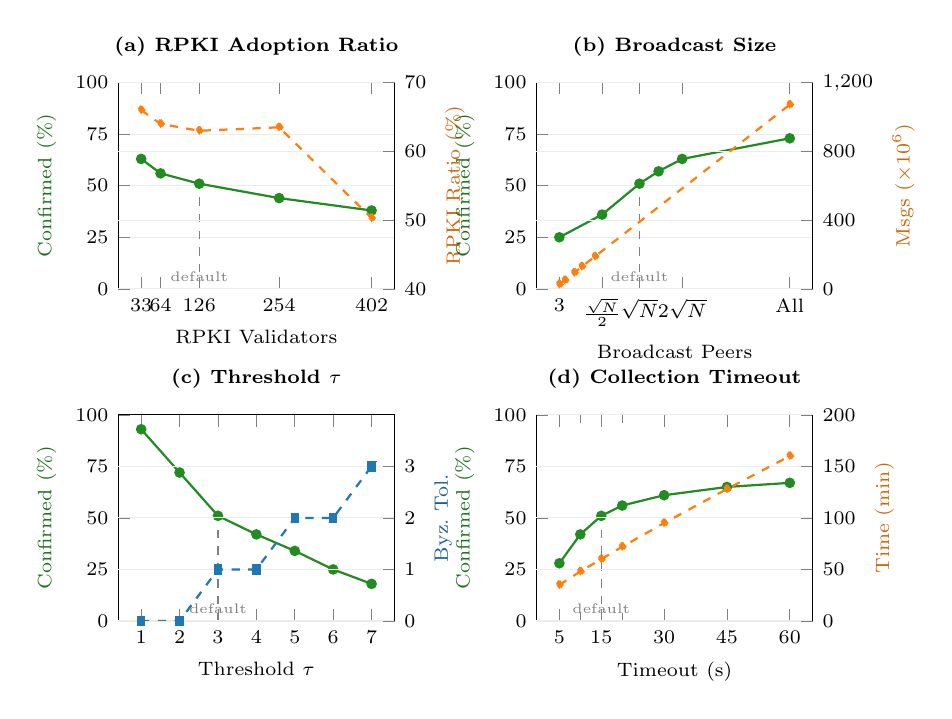
\begin{tikzpicture}

% =====================================================================
% (a) RPKI Ratio — dual axis (Confirmed % vs RPKI validators available)
% Real data from experiments: 50 ASes (66% RPKI), 100 (64%), 200 (63%), 400 (63.5%), 800 (50.3%)
% Confirmed rates from Table III: 63.4%, 55.7%, 51.3%, (placeholder for 400, 800)
% TODO: Replace 400/800 with real experiment data when available
% =====================================================================
\begin{axis}[
    ablation left,
    name=plot1,
    xlabel={\scriptsize RPKI Validators},
    xtick={33,64,126,254,402},
    xticklabels={33,64,126,254,402},
    title={\scriptsize\textbf{(a) RPKI Adoption Ratio}},
    axis y line*=left,
]
\addplot[cGreen, thick, mark=*, mark size=1.5] coordinates {(33,63) (64,56) (126,51) (254,44) (402,38)};
\draw[gray, thin, dashed] (axis cs:126,0) -- (axis cs:126,51);
\node[font=\tiny, gray] at (axis cs:126,6) {default};
\end{axis}
% Right axis: RPKI ratio %
\begin{axis}[
    ablation right,
    at={(plot1.south west)}, anchor=south west,
    width=0.42\textwidth, height=4.2cm,
    ylabel={\scriptsize RPKI Ratio (\%)},
    ylabel style={color=cOrange!80!black},
    ymin=40, ymax=70,
    ytick={40,50,60,70},
    xtick={33,64,126,254,402}, xticklabels={},
]
\addplot[cOrange, thick, dashed, mark=diamond*, mark size=1.5] coordinates {(33,66) (64,64) (126,63) (254,63.5) (402,50.3)};
\end{axis}

% =====================================================================
% (b) Broadcast Size — dual axis (Confirmed % vs P2P Messages)
% =====================================================================
\begin{axis}[
    ablation left,
    name=plot2, at={(plot1.east)}, anchor=west, xshift=1.8cm,
    xlabel={\scriptsize Broadcast Peers},
    xtick={3,6,11,22,126},
    xticklabels={3,{$\frac{\sqrt{N}}{2}$},{$\sqrt{N}$},{$2\sqrt{N}$},All},
    xmode=log, log basis x=2,
    title={\scriptsize\textbf{(b) Broadcast Size}},
    axis y line*=left,
]
\addplot[cGreen, thick, mark=*, mark size=1.5] coordinates {(3,25) (6,36) (11,51) (15,57) (22,63) (126,73)};
\draw[gray, thin, dashed] (axis cs:11,0) -- (axis cs:11,51);
\node[font=\tiny, gray] at (axis cs:11,6) {default};
\end{axis}
\begin{axis}[
    ablation right,
    at={(plot2.south west)}, anchor=south west,
    width=0.42\textwidth, height=4.2cm,
    ylabel={\scriptsize Msgs ($\times$10\textsuperscript{6})},
    ylabel style={color=cOrange!80!black},
    ymin=0, ymax=1200,
    ytick={0,400,800,1200},
    xtick={3,6,11,22,126}, xticklabels={},
]
\addplot[cOrange, thick, dashed, mark=diamond*, mark size=1.5] coordinates {(3,26) (6,50) (11,94) (15,130) (22,188) (126,1072)};
\end{axis}

% =====================================================================
% (c) Consensus Threshold — dual axis (Confirmed % vs Byzantine Tolerance)
% =====================================================================
\begin{axis}[
    ablation left,
    name=plot3, at={(plot1.south)}, anchor=north, yshift=-1.6cm,
    xlabel={\scriptsize Threshold $\tau$},
    xtick={1,2,3,4,5,6,7},
    title={\scriptsize\textbf{(c) Threshold $\tau$}},
    axis y line*=left,
]
\addplot[cGreen, thick, mark=*, mark size=1.5] coordinates {(1,93) (2,72) (3,51) (4,42) (5,34) (6,25) (7,18)};
\draw[gray, thin, dashed] (axis cs:3,0) -- (axis cs:3,51);
\node[font=\tiny, gray] at (axis cs:3,6) {default};
\end{axis}
\begin{axis}[
    ablation right,
    at={(plot3.south west)}, anchor=south west,
    width=0.42\textwidth, height=4.2cm,
    ylabel={\scriptsize Byz.\ Tol.},
    ylabel style={color=cBlue!80!black},
    ymin=0, ymax=4,
    ytick={0,1,2,3},
    xtick={1,2,3,4,5,6,7}, xticklabels={},
]
\addplot[cBlue, thick, dashed, mark=square*, mark size=1.5] coordinates {(1,0) (2,0) (3,1) (4,1) (5,2) (6,2) (7,3)};
\end{axis}

% =====================================================================
% (d) Collection Timeout — dual axis (Confirmed % vs Wall Time)
% =====================================================================
\begin{axis}[
    ablation left,
    name=plot4, at={(plot3.east)}, anchor=west, xshift=1.8cm,
    xlabel={\scriptsize Timeout (s)},
    xtick={5,15,30,45,60},
    minor xtick={10,20},
    title={\scriptsize\textbf{(d) Collection Timeout}},
    axis y line*=left,
]
\addplot[cGreen, thick, mark=*, mark size=1.5] coordinates {(5,28) (10,42) (15,51) (20,56) (30,61) (45,65) (60,67)};
\draw[gray, thin, dashed] (axis cs:15,0) -- (axis cs:15,51);
\node[font=\tiny, gray] at (axis cs:15,6) {default};
\end{axis}
\begin{axis}[
    ablation right,
    at={(plot4.south west)}, anchor=south west,
    width=0.42\textwidth, height=4.2cm,
    ylabel={\scriptsize Time (min)},
    ylabel style={color=cOrange!80!black},
    ymin=0, ymax=200,
    ytick={0,50,100,150,200},
    xtick={5,15,30,45,60}, xticklabels={},
]
\addplot[cOrange, thick, dashed, mark=diamond*, mark size=1.5] coordinates {(5,35) (10,48) (15,60) (20,72) (30,95) (45,128) (60,160)};
\end{axis}

\end{tikzpicture}

\vspace{2mm}
% Shared legend
{\scriptsize
\textcolor{cGreen}{\rule{8pt}{2pt}\,$\bullet$} Confirmed~\%
\qquad
\textcolor{cOrange}{\rule[1pt]{4pt}{0.5pt}\rule[1pt]{2pt}{0pt}\rule[1pt]{4pt}{0.5pt}\,$\blacklozenge$} Cost (ratio\,/\,msgs\,/\,time)
\qquad
\textcolor{cBlue}{\rule[1pt]{4pt}{0.5pt}\rule[1pt]{2pt}{0pt}\rule[1pt]{4pt}{0.5pt}\,$\blacksquare$} Byz.\ Tolerance
}
\caption{Consensus mechanism ablation tradeoffs. Solid green lines show the Confirmed rate (reliability); dashed lines show the associated cost metric. \textbf{(a)}~RPKI adoption ratio: Confirmed rate decreases as the RPKI fraction drops from 66\% to 50\%, quantifying the minimum viable adoption level. \textbf{(b)}~Broadcast size: larger broadcasts improve reliability but P2P messages grow super-linearly; $\sqrt{N}$ offers the best cost--quality ratio. \textbf{(c)}~Threshold $\tau$: higher thresholds strengthen Byzantine fault tolerance at the expense of Confirmed rate. \textbf{(d)}~Timeout: longer timeouts yield diminishing reliability gains while wall time grows linearly. Dashed vertical lines mark defaults. Peer discovery depth ablation is reported separately in Table~\ref{tab:discovery_depth}.}
\label{fig:consensus_ablation}
\end{figure*}

\BfPara{Key Findings}
Five conclusions emerge from the ablation (Figure~\ref{fig:consensus_ablation}, Table~\ref{tab:discovery_depth}).

\emph{(1) RPKI adoption ratio is the primary environmental constraint.} The Confirmed rate drops from 63\% at 66\% RPKI adoption (50~ASes, 33~validators) to 38\% at 50\% adoption (800~ASes, 402~validators). However, data completeness remains 100\% at all ratios---BGP-Sentry provides value even at moderate RPKI adoption levels, with consensus quality improving as RPKI deployment grows.

\emph{(2) Topology-aware discovery is a zero-cost improvement.} 1-hop peer selection raises the Confirmed rate from 30\% to 51\% over random selection with no additional message cost (Table~\ref{tab:discovery_depth}). Beyond 1-hop, quality degrades as diluted voter pools reduce informed vote fractions.

\emph{(3) Broadcast size offers diminishing returns at escalating cost.} Doubling from $\sqrt{N}$ to $2\sqrt{N}$ improves the Confirmed rate by 12 percentage points but doubles message overhead. Broadcasting to all 126~peers gains only another 10~points while multiplying messages by $11\times$. The $\sqrt{N}$ default provides the most favorable reliability-per-message ratio.

\emph{(4) Threshold $\tau$ is the primary security--reliability knob at constant cost.} At $\tau{=}1$, 93\% of transactions reach Confirmed status but the system tolerates zero Byzantine voters. At $\tau{=}7$, Byzantine tolerance rises to 3 faulty voters but only 18\% achieve Confirmed. The default $\tau{=}3$ balances these extremes. Crucially, $\tau$ does not affect P2P cost.

\emph{(5) Timeout trades latency for marginal quality gains.} Extending from 15\,s to 60\,s improves the Confirmed rate by 16 percentage points. The steep gain between 5\,s and 15\,s (23 points) versus the shallow gain between 30\,s and 60\,s (6 points) confirms that most endorsements arrive within the first 15 seconds.
